\chapter{Analog/Mixed-signal Design Approach}
\begin{figure}[h]
\begin{center}
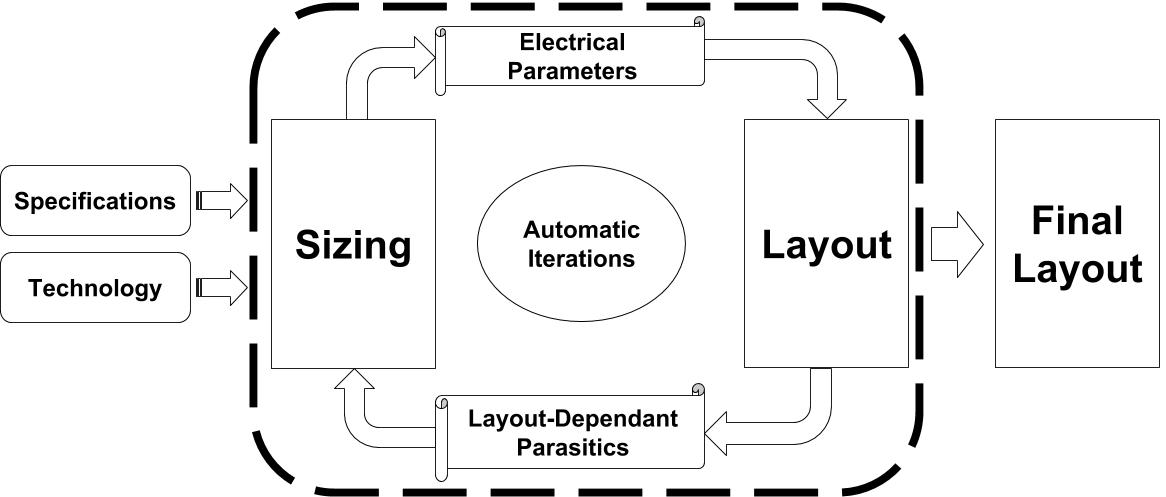
\includegraphics[height=40mm]{Figures/3.jpg}
\caption{Cairo Hurricane AMS Design Flow}
\end{center}
\end{figure}
\vspace{-1.5cm}
\section{Design Flow}
The Cairo Hurricane AMS (CHAMS) project cite{002}, developed by the LIP6 Laboratory, proposes a complete flow which would be able to create a library of reconfigurable analog Intellectual Properties, to automatically generate and optimize the layout with little intervention from the designer. The flow provides a reliable and efficient solution taking into account parasitic effect-aware layout generation with enough flexibility to adapt to different designers needs and concerns. CHAMS layout generation tool supports any technology with the new nanometric layout dependent parasitic parameters.
\newline 
\newline 
\indent The proposed CHAMS analog design (Fig. 2) is a two way communication between the sizing and layout generation. The idea is that the sizing tool provides the electrical parameters of the transistor such as the width, length, number of fingers, etc... to the layout generation tool. The tool automatically generates the layout from a library of parameterized cells and sends back to the sizing engine the layout-dependent parasitic parameters such as the drain and source areas and perimeters, the stress effect parameters, etc... to re-evaluate the performance. This internal loop is repeated several times, with minimal designer intervention, until the target specifications are met.
\newline 
\newline 
\indent Our goal is to develop a tool capable to place and route analog layout respecting designer specifications in a shorter amount of time compared to the fully manual approach. We also aim to have a tool which will be technology independant and can as well, place  and route mixed-signal circuits. At this moment, the bottleneck of our design flow is to handle analog place and route and this is the reason why this thesis is mainly focused on it.
 
\section{Placement in row}
Digital and analog circuits have a dedicated area on a system-on-chip circuit so they can be independently designed within a specific space. Digital circuits are well-known for their regular row structure where standard cells are placed and routed accordingly to their netlist. In a similar way, we plan to organize the analog circuit layout in rows of devices and the analog circuit area should be placed and routed within its dedicated area. 
\newline 
\newline 
\indent It is common to design analog circuit in rows of devices where the height of each row of devices should be adjustable so it can match its dedicated area. Therefore, we choose the slicing tree representation for several reasons:

\begin{itemize}
\item Slicing trees are a natural choice since they are adequate to the row structure. Rows are represented by horizontal slices which will be divided into vertical slices determined by the area of each device.

\item Unlike most of modern analog placement methods, our placement strategy is semi-automatic and will be guided by the designer's preferences. Slicing trees are easy to handle and let the designer choose the overall topology. That shows some advantages that will be explained in the following section.
\end{itemize}